% Generated by revision/reporting.py -- paste into the manuscript and edit.
% Copy figures/*.pdf next to main.tex (vector PDF; do not use the PNGs).

\begin{figure}[t]
\centering
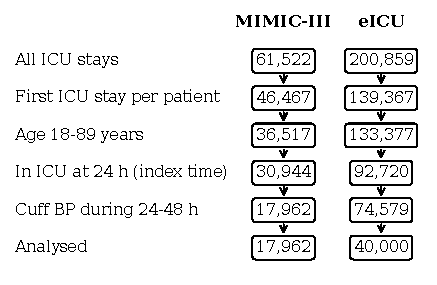
\includegraphics[width=\columnwidth]{fig_cohort_flow.pdf}
\caption{Cohort selection in MIMIC-III and eICU. The unit of analysis is the first ICU stay per patient. Index time is 24 h after ICU admission; the prediction target is non-invasive (cuff) blood pressure during hours 24-48. eICU was reduced to a deterministic random sample of 40,000 stays for computational reasons.}
\label{fig:cohort_flow}
\end{figure}

\begin{figure*}[t]
\centering
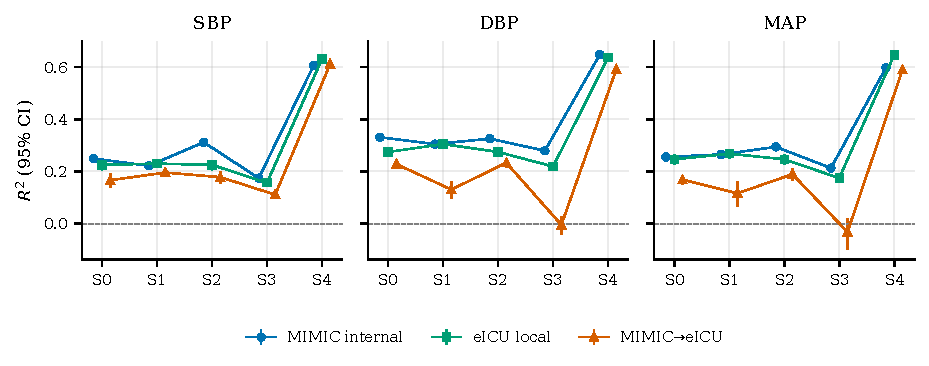
\includegraphics[width=\textwidth]{fig_harmonization_ladder.pdf}
\caption{Harmonization ladder: $R^2$ (95\% CI) for SBP, DBP and MAP as one analysis choice is changed at a time. S0, the submitted task (features and target from the same window; MIMIC-III any BP modality, eICU arterial line); S1, cuff BP in both datasets; S2, arterial BP in both; S3, prospective task (features 0-24 h, target 24-48 h) without BP history; S4, S3 with observation-window BP history. MIMIC internal and eICU local use patient-grouped 5-fold cross-validation; MIMIC$\rightarrow$eICU trains on all MIMIC-III stays. CIs from 1,000 bootstrap resamples (patients for MIMIC-III, hospitals for eICU).}
\label{fig:harmonization_ladder}
\end{figure*}

\begin{figure*}[t]
\centering
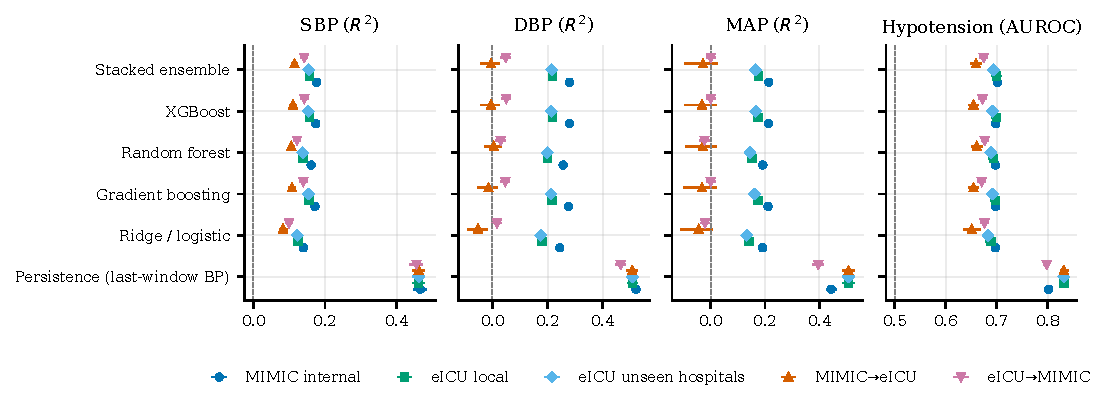
\includegraphics[width=\textwidth]{fig_models_transfer.pdf}
\caption{Discrimination of all models under five validation settings: MIMIC-III internal, eICU local (patient-grouped cross-validation), eICU unseen hospitals (hospital-grouped cross-validation), MIMIC-III$\rightarrow$eICU and eICU$\rightarrow$MIMIC-III. $R^2$ for SBP, DBP and MAP; AUROC for hypotension ($\geq$2 hourly MAP values $<$65 mmHg during hours 24-48). Persistence predicts the observation-window BP. Bars show 95\% bootstrap CIs.}
\label{fig:models_transfer}
\end{figure*}

\begin{figure*}[t]
\centering
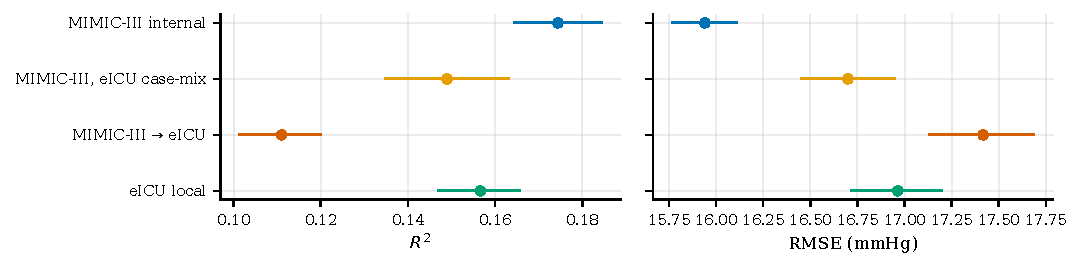
\includegraphics[width=\textwidth]{fig_gap_decomposition_sbp.pdf}
\caption{Decomposition of the MIMIC-III$\rightarrow$eICU performance gap for SBP. ``eICU case-mix'' reweights held-out MIMIC-III predictions by the estimated density ratio so the covariate distribution matches eICU (performance expected under pure covariate shift); the remaining difference to MIMIC-III$\rightarrow$eICU reflects a change in the feature--BP relationship. eICU local is the achievable reference.}
\label{fig:gap_decomposition_sbp}
\end{figure*}

\begin{figure*}[t]
\centering
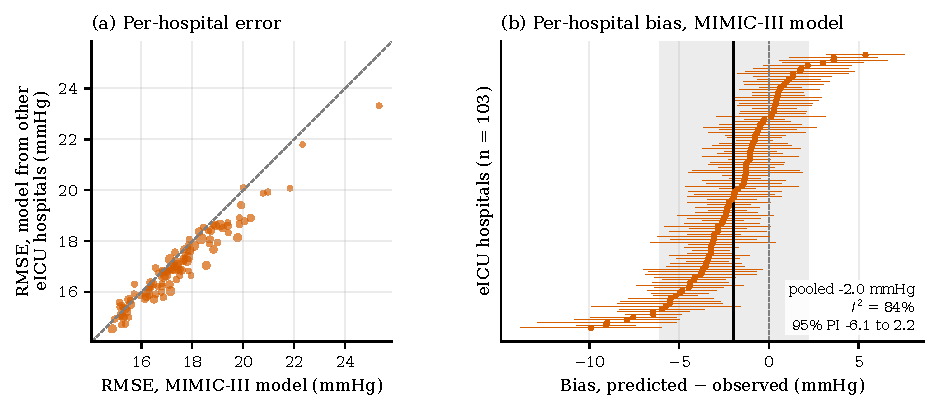
\includegraphics[width=\textwidth]{fig_hospitals_sbp.pdf}
\caption{Per-hospital performance in eICU hospitals with $\geq$100 stays. (a) RMSE of the MIMIC-III model versus a model trained on other eICU hospitals (hospital-grouped cross-validation); points on the diagonal indicate no MIMIC-specific transfer loss; point size reflects the number of stays. (b) Mean prediction bias of the MIMIC-III model per hospital (95\% CI), with the random-effects pooled estimate, heterogeneity ($I^2$) and 95\% prediction interval.}
\label{fig:hospitals_sbp}
\end{figure*}

\begin{figure}[t]
\centering
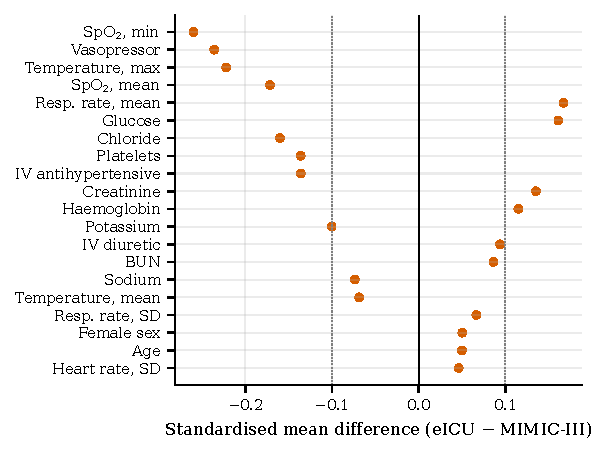
\includegraphics[width=\columnwidth]{fig_feature_shift.pdf}
\caption{Standardised mean differences of the model features between eICU and MIMIC-III (dotted lines at $\pm$0.1).}
\label{fig:feature_shift}
\end{figure}

\begin{figure*}[t]
\centering
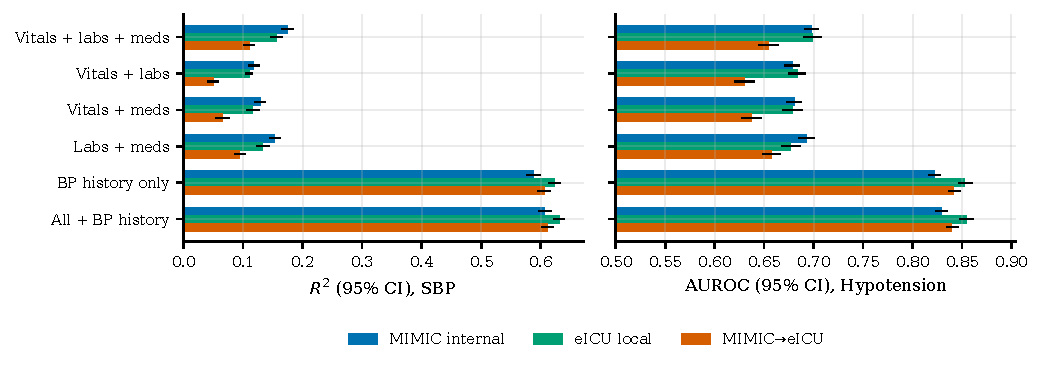
\includegraphics[width=\textwidth]{fig_feature_ablation.pdf}
\caption{Feature-set ablation on a fixed cohort (every feature set is evaluated on the same patients): $R^2$ for SBP and AUROC for hypotension, 95\% bootstrap CIs. ``All + BP history'' is the clinically relevant forecasting model.}
\label{fig:feature_ablation}
\end{figure*}

\begin{figure*}[t]
\centering
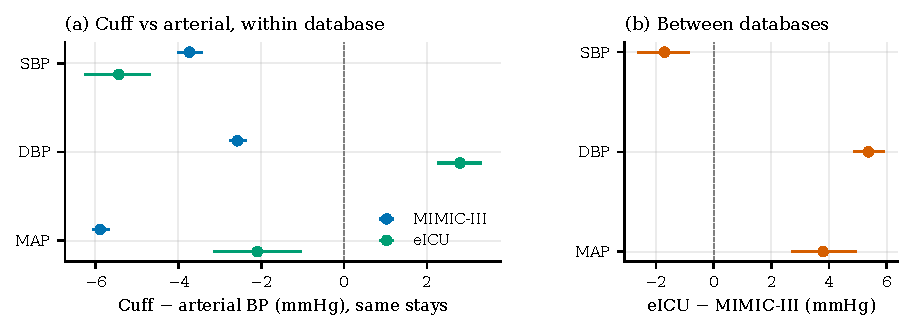
\includegraphics[width=\textwidth]{fig_modality_agreement.pdf}
\caption{Cuff versus arterial blood pressure in stays with both measurements during the first 24 h (window means; not time-matched pairs). (a) Mean cuff minus arterial difference within each database. (b) Between-database difference in (a); a non-zero value indicates that cuff pressures are measured or recorded differently, since arterial pressures agree across databases. 95\% cluster-bootstrap CIs.}
\label{fig:modality_agreement}
\end{figure*}

\begin{figure*}[t]
\centering
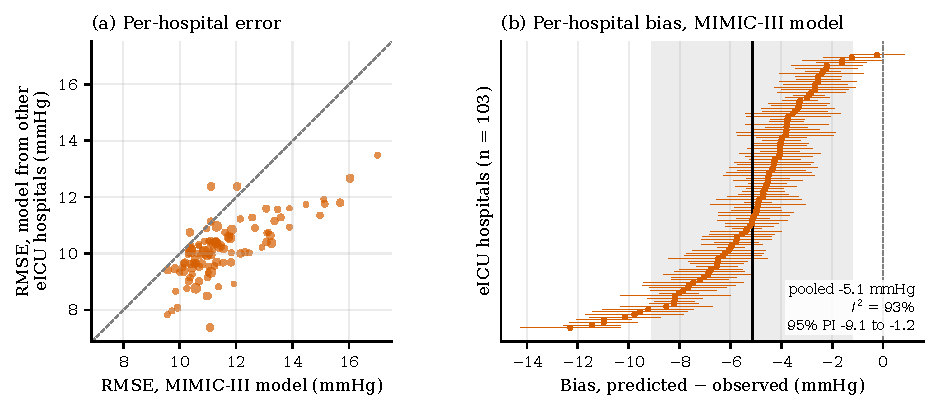
\includegraphics[width=\textwidth]{fig_hospitals_dbp.pdf}
\caption{As Fig.~\ref{fig:hospitals_sbp}, for diastolic blood pressure.}
\label{fig:hospitals_dbp}
\end{figure*}

\begin{figure}[t]
\centering
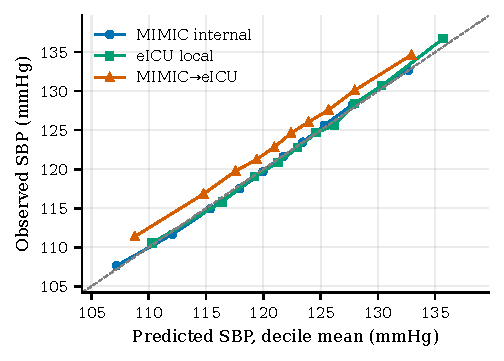
\includegraphics[width=\columnwidth]{fig_calibration_sbp_xgb.pdf}
\caption{Calibration of SBP predictions (XGBoost): observed versus predicted SBP by decile of predicted value. The dashed line is perfect calibration.}
\label{fig:calibration_sbp_xgb}
\end{figure}
